%%%%%%%%%%%%%%%%%%%%%%%%%%%%%%%%%%%%%%%%%%%%%%%%%%%%%%%%%%%%%%%%%%%%%%%%%%%%%%%%
%                                                                              %
%                                                                              %
%                                                                              %
%%%%%%%%%%%%%%%%%%%%%%%%%%%%%%%%%%%%%%%%%%%%%%%%%%%%%%%%%%%%%%%%%%%%%%%%%%%%%%%%

% A4, double-sided, font 12pt
\documentclass[a4paper,12pt,twoside]{report}

\usepackage[top=3.81cm,bottom=3cm,inner=3.5cm,outer=2.54cm]{geometry}

% Actual font selection
\usepackage{pxfonts} % bookman | pxfonts | cmbright

% Include support for romanian hyphenation (if installed on your sistem)
\usepackage[romanian]{babel}

% Include support for correct printing of romanian characters
\usepackage[T1]{fontenc}
\usepackage{ucs}
\usepackage[utf8x]{inputenc}

% Include support for graphics
\usepackage[pdftex]{color,graphicx}

% Include support for columns
\usepackage{multicol}

% Text alignment
\usepackage{ragged2e}

\usepackage{floatrow}

\usepackage{tabularx}
\renewcommand\tabularxcolumn[1]{>{\Centering}m{#1}}

% Include support for hyperlinks in the document
\usepackage{hyperref}
\hypersetup{unicode=true,%
	colorlinks=true,%
	citecolor=black,%
	filecolor=black,%
	linkcolor=black,%
	urlcolor=black}

\setcounter{tocdepth}{3}

% Simboluri grecești
\usepackage{upgreek}

% Indent first paragraph
\usepackage{indentfirst}

% Appendices
\usepackage[titletoc]{appendix}

% Paragraph
\usepackage{parskip}
\setlength{\parindent}{2em}

% Comandă inserare figură
\newcommand{\insfig}[4]{
	\begin{figure}[!htb]
		\begin{center}
			\includegraphics[width=#4\textwidth]{figuri/#1}
			\caption{#2\label{#3}}
	    \end{center}
	\end{figure}
}

% Comandă inserare figură cu sursă
\newcommand{\insfigs}[5]{
	\begin{figure}[!htb]
		\begin{center}
			\includegraphics[width=#5\textwidth]{figuri/#1}
			\caption[#2 \-\ \-\ \-\ \-\ \-\ \-\ \-\ \-\ \-\ \-\ \-\ \-\ \-\ \-\ \-\ \-\ 
			\-\ \-\ \-\ \-\ \-\ \-\ \-\ \-\ \protect\linebreak Sursa: #3]{#2\label{#4}}
	    \end{center}
	\end{figure}
}

% Setting headers
\usepackage{fancyhdr}
\pagestyle{fancy}
\fancyhead{}
\fancyhead[LE]{\nouppercase{\leftmark}}
\fancyhead[RO]{\nouppercase{\rightmark}}

% Set spacing at 1.5lines
\linespread{1.2}

% Document begins here
\begin{document}

% Create title page
\thispagestyle{empty}
\begin{center}

{\large
    UNIVERSITATEA POLITEHNICA DIN BUCUREȘTI \\
    FACULTATEA DE AUTOMATICĂ ȘI CALCULATOARE \\
    DEPARTAMENTUL DE CALCULATOARE \\
}

\vspace{\stretch{1}}

\begin{tabular}{m{0.28\linewidth}m{0.4\linewidth}m{0.22\linewidth}}
%\flushleft 
\center 
\includegraphics[height=2.2cm]{figuri/upb-logo.png} &
\center 
\includegraphics[height=2.2cm]{figuri/cs-logo.png} &
%\flushright 
\center 
\includegraphics[height=2.6cm]{figuri/acs-logo.png}
\end{tabular}

\vspace{\stretch{12}}

{\LARGE
	\textbf{LUCRARE DE DIPLOMĂ}\\
	\vspace{\stretch{3}}
	\textbf{Robot Explorator}
}

\vspace{\stretch{8}}

{\large
    \begin{multicols}{2}
        \begin{flushleft}
        \textbf{Coordonatori științifici:}\\
        Prof.dr.ing. Mariana Mocanu\\
        \fbox{Prof.dr.ing. Șerban Petrescu}
        \end{flushleft}
    \columnbreak
        \begin{flushright}
        \textbf{Absolvent:}\\
        Bogdan Folea
        \end{flushright}
    \end{multicols}
}

\vspace{\stretch{20}}

{\large
    \textbf{BUCUREȘTI\-\ \-\ \-\ }\\
    - 2017 -
}

\end{center}


% Leave a blank page for double side printing
%\thispagestyle{empty}
%\newpage
%\hbox{}

% Abstract
\thispagestyle{empty}
\begin{flushleft}

\vspace*{100px}

\justify\large\textit{
    Lucrarea de față are în vedere proiectarea, asamblarea și programarea unui robot telecomandat semiautonom având la bază un sistem de operare în timp real, cu scopul de a colecta informații despre mediul înconjurător și a le transmite mai departe către un calculator. Acest lucru a fost realizat în scopul explorării unor medii în care accesul uman este restricţionat.
}

\end{flushleft}


% Leave a blank page for double side printing
%\thispagestyle{empty}
%\newpage
%\hbox{}

% Cuprins
\newpage
\setcounter{page}{1}
{\large
    \tableofcontents
}

% Capitole
\chapter{Introducere}

Istoria roboților își are originile în Antichitatea clasică, fapt dovedit de scrierile matematicianului Heron din Alexandria, care stau mărturie existenței unor mecanisme automate \cite{heron} bazate pe principii mecanice. Fascinația pentru construcția unor astfel de mecanisme s-a manifestat și în perioada Renașterii italiene, prin schițele lui Leonardo da Vinci și mai târziu în timpul Revoluției Industriale.

Momentul de cotitură în acest domeniu îl constituie dezvoltarea electronicii și apariția circuitelor integrate digitale, în urma căruia a s-a cristalizat știința care se ocupă cu proiectarea, construcția și operarea roboților, precum și sistemele de control, reacție la stimuli exteriori și procesare a informației, sub numele de robotică.

Această ramură a tehnicii a cunoscut o ascensiune vizibilă în trecutul recent, o dată cu apariția Inteligenței Artificiale și a Internetului Obiectelor (\textit{engl. IoT}\footnote{Internet of Things}), conducând efectiv la integrarea circuitelor electronice cu sitemul de locomoție al robotului și posibilitatea de a conecta între ele mai multe astfel de sisteme autonome prin intermediul diverselor protocoale de comunicații.

În prezent, datorită progreselor rapide înregistrate în domeniu, roboții au ajuns să îndeplinească funcții din ce în ce mai diverse. Printre acestea se numără fabricarea de automobile, unde au ajuns să aibă o pondere tot mai mare, sub forma liniilor de producție complet automatizate, au ajuns să aibă o pondere tot mai mare pe parcursul ultimelor decenii. De asemenea, roboții au ajuns să fie folosiți extensiv și la împachetarea produselor alimentare, transportul mărfurilor în interiorul spațiilor de depozitare, recolta anumitor culturi de fructe, fabricarea cablajelor imprimate, precum și în exploatări miniere. Pe lângă tipurile de roboți industriali enumerate mai devreme, s-au dezvoltat roboți care pot duce independent la îndeplinire sarcini domestice ca tunsul ierbii sau aspirarea covoarelor și, nu în ultimul rând, roboți umanoizi, care au scopul de a imita comportamentul oamenilor sau părți din acesta, de exemplu mersul biped.

Spre deosebire de situațiile menționate anterior, unde roboții sunt folosiți cu scopul de a spori productivitatea unor activități ce pot fi efectuate de agenți umani, există împrejurări, care, prin natura lor, care impun folosirea unui robot. Poate cel mai bun exemplu este explorarea mediilor fizic inaccesibile oamenilor, aflate la mare distanță sau  având indici de risc care depășesc valori considerate admise, punând astfel în pericol o eventuală intervenție umană. Câteva exemple sunt interiorul conductelor, spațiul cosmic și mediile vulcanice sau puternic radioactive. Roboții special construiți cu scopul de a explora astfel de medii se încadrează în categoria roboților exploratori.


\section{Motivație}

Nivelul actual de dezvoltare a roboticii conduce la o popularitate în creștere a roboților exploratori în rândul comunității științifice și inginerești. Fie că este vorba despre roboți exploratori tereștri, sateliți artificiali sau drone, utilitățile acestora sunt nenumărate și se reflectă în numărul impresionant de cercetări privind explorarea spațiilor de orice natură și fascinația pe care o exercită asupra unei vaste categorii de oameni. Caracteristice acestor roboți sunt sistemele complicate necesare pentru a îndeplini chiar sarcini foarte simple, acoperind o multitudine de discipline diferite printre care se numără mecanica, electronica, telecomunicațiile și programarea.

La baza complexității roboților exploratori stă o varietate de constrângeri care se manifestă în moduri diferite în fiecare caz în parte. În particular, o dronă are nevoie de măsurători foarte precise ale înclinării și accelerației, precum și de un metodă eficientă de anulare a zgomotului, în timp ce calitatea cea mai importantă a unui robot destinat explorării spațiului cosmic este fiabilitatea. Un exemplu elocvent în acest caz este robotul \textit{Curiosity} al Agenției Spațiale Americane (\textit{engl. NASA}\footnote{National Aeronautics and Space Administration}), lansat în noiembrie 2011 pentru a explora planeta Marte.

\insfigs{curiosity.jpg}{Robotul explorator \textit{Curiosity} al NASA}{\href{https://www.jpl.nasa.gov/spaceimages/details.php?id=PIA09201}{www.jpl.nasa.gov} (15.05.2017)}{curiosity}{0.6}

La doar șase luni de la aterizarea acestuia, o eroare în memoria pilotului principal, combinată cu defectarea simultană a mecanismelor de siguranță a condus la un potențial dezastru \cite{curiosity} însemnând pierderea definitivă a întregii investiții de 2,5 miliarde de dolari americani.

Comună tuturor sistemelor mai sus amintite este constrângerea de timp real (\textit{engl. real-time constraint}) la care sunt supuse, definită garanția răspunsului la un stimul exterior înaintea unui termen limită prestabilit, indiferent de încărcarea sistemului. Soluția elegantă la această problemă este oferită de sistemele de operare în timp real (\textit{engl. RTOS}\footnote{Real-Time Operating System}).

Dezvoltarea în ultimul deceniu a sistemelor de operare în timp real se datorează în mare parte creșterii puterii de procesare a microcontrollerelor, rezultând în folosirea mai eficientă a timpului de calcul. Întrucât o schimbare de context\footnote{Schimbarea execuţiei unui proces cu un altul pe procesor} durează foarte puțin (ordinul microsecundelor), sistemele de operare actuale nu mai sunt constrânse de frecvența cu care apare, ceea ce conduce la un timp de răspuns îmbunătățit semnificativ.

În momentul de față există o multitudine de astfel de sisteme de operare, sub licență proprietară sau open source. Dintre acestea din urmă cel mai popular este \textit{FreeRTOS}, dezvoltat de \textit{Real Time Engineers Ltd.}, a cărui descriere detaliată se găsește în lucrarea de față la capitolul aferent. Acesta prezintă un număr mare de avantaje care îl recomandă, printre care faptul că e orientat pe evenimente, simplitatea interfeței de acces (\textit{engl. API}\footnote{Application Programming Interface}), documentația clară și abundentă, precum și suportul on-line de calitate.

Posibilitatea de a utiliza acest sistem de operare în timp real, flexibil și asincron, la baza unui robot explorator în scopul de a folosi eficient timpul de calcul și a obține un timp bun de răspuns la comenzi sau stimuli exteriori constituie motivația din spatele realizării acestui proiect.


\section{Scopul lucrării}

Lucrarea de față are drept scop proiectarea, asamblarea și programarea unui robot explorator operat de la distanță, destinat mediului terestru. Acesta trebuie să măsoare o varietate de parametri caracteristici mediului înconjurător precum temperatura, presiunea, umiditatea și intensitatea luminii ambientale și să transmită datele operatorului. În plus, este necesar ca acesta să reacționeze autonom în situații de risc ce îi pun în pericol integritatea. Găsirea unei modalități eficiente de a garanta că atât răspunsul la comenzile de deplasare, cât și transferul continuu al datelor se petrec în timp real, face, de asemenea, obiectul acestei lucrări.


\section{Stadiul actual}

Un robot destinat explorării terestre este dotat cu roți sau, cel mai frecvent, montat pe un șasiu cu șenile, ceea ce îi conferă mobilitate și stabilitate crescută pe terenuri accidentate și facilitează ocolirea sau depășirea eventualelor obstacole. Un exemplu în acest sens este robotul \textit{Urbie Rover} al NASA.

\insfigs{urbie.jpg}{Robotul urban \textit{Urbie Rover} al NASA}{\href{https://www.jpl.nasa.gov/news/news.php?feature=485}{www.jpl.nasa.gov}  (16.05.2017)}{urbie}{0.6}

Acesta servește în special la explorarea mediilor urbane, caracterizate de obstacole dificil de trecut ca serii de trepte sau borduri. Este prevăzut cu șenile, wireless Ethernet, receptor GPS diferențial, busolă digitală, LIDAR\footnote{Light Imaging, Detection, And Ranging}, o cameră de luat vederi omnidirecțională, o pereche de camere video pentru vedere binoculară și două procesoare Intel Pentium PC-104. Arhitectura sa este una modulară, unul din procesoare fiind rezervat pentru navigație, iar celălalt pentru procesarea de imagini. Aceste echipamente îi oferă posibilitatea de a îndeplini autonom o varietate de sarcini, precum localizarea în spațiu, urcarea treptelor, evitarea obstacolelor și reconstituirea și retraversarea traseului parcurs.

Cu certitudine se poate spune că, în această categorie, cei mai utili sunt roboții proiectați să opereze în spații de dimensiuni reduse, spre exemplu în interiorul unor conducte de ventilație, cu scopul de a localiza posibile defecte sau chiar în scopul cercetărilor arheologice. Elocvent în acest sens este cazul robotului explorator \textit{Djedi}, dezvoltat de comunitatea internațională de egiptologi în colaborare cu Universitatea din Leeds.

\insfigs{djedi.png}{Robotul explorator \textit{Djedi}}{\href{http://archive.archaeology.org/1109/trenches/djedi_project_robot_pyramid_khufu_palenque.html}{archive.archaeology.org} (20.05.2017)}{djedi}{0.6}

Un caz aparte, \textit{Djedi} a fost special proiectat și construit în scopul de a explora puțurile de ventilație din Marea Piramidă a lui Kheops \cite{djedi}, un exemplu excelent de problemă pentru care utilizarea unui robot este unica soluție, explorarea acestui mediu fiind cu desăvârșire imposibil de realizat folosind orice altă metodă.


\section{Sisteme embedded}

Sistemul expus în lucrarea de față intră în categoria sistemelor încorporate sau \textit{embedded} în timp real, dedicate doar rezolvării unui anumit tip de sarcini și atingerii simultane a unor țeluri cuantificabile. Este necesar ca la proiectarea unui astfel de sistem să se țină seama de aceste țeluri, din care cel mai important este garanția răspunsului în timp real, dar printre care se numără și consumul de energie și, nu în ultimul rând, costul. Cerințele specifice conduc inevitabil la compromisuri diferite între performanță și consumul de energie sau accentul predominant pus pe hardware sau software.

Contrastând puternic cu calculatoarele de uz general, unde nu se cunoaște în prealabil modul în care vor fi folosite și ale căror arhitecturi trebuie să permită folosirea lor în feluri cât mai diverse, în cazul unui sistem embedded atât proiectarea hardware cât și software se realizează simultan. Prin urmare, o problemă întâmpinată poate fi rezolvată în hardware, software sau o combinație între cele două. Aceste abordări implică compromisuri diferite, deci oferă un spațiu mai mare de manevră și posibilitatea de a obține o soluție calitativ mai bună, mai fiabilă și flexibilă, fără însă de a prezenta flexibilitate inutil de mare în detrimentul îndeplinirii cerințelor. \cite{wolf}

Un sistem embedded operează în timp real atâta timp cât execută procesele critice într-un timp acceptabil. Definiția flexibilă a acestui interval îl încadrează ca parte a cerințelor comportamentale ale sistemului și nu a celor funcționale. Este obligatoriu ca aceste cerințe să fie măsurabile sau cuantificabile în mod obiectiv, dar pot fi reduse la un model de administrare a resurselor ce poate fi statică sau dinamică, aflată în sarcina unui programator, respectiv a unui sistem de operare. Administrarea resurselor în timp real are însă asociat un cost, deoarece este imposibil de obținut gradul de încredere într-un timp rezonabil de răspuns doar prin redimensionarea hardware-ului. În contextul interacțiunii cu alte dispozitive, un sistem embedded are nevoie atât de capabilități hardware adecvate, cât și de eficiență în administrarea software a resurselor. Mediul este complex și în continuă schimbare și acest lucru se reflectă în numărul și ponderea interacțiunilor. Importanța maximă în acest context aparține evaluării corecte a timpului fizic, necesară pentru a corela evenimentele cu momentele exacte ale producerii lor, nu cea logică, asupra căreia sistemele au în mod automat control. Prin urmare, caracteristica esențială a sistemelor embedded în timp real devine inevitabil găsirea unui compromis între performanță și timpul definit ca acceptabil. \cite{kraeling}


\chapter{Arhitectura hardware}

Arhitectura hardware propusă este una modulară și prevede, în măsura în care acest lucru este posibil, componente diferite pentru a îndeplini funcții diferite. Întregul sistem este proiectat în jurul unei unități responsabile de controlul robotului, reprezentată de un microcontroller (MCU) capabil de a satisface constrângerea de timp real.

\insfig{bloc.png}{Schema bloc a sistemului}{bloc}{0.9}

Direct conectați la aceasta sunt o serie de senzori de mai multe tipuri, reprezentând o importantă parte a sistemului deoarece oferă informații vitale despre mediul înconjurător, subansamblul responsabil cu locomoția, format din motoare și puntea de control montate pe un șasiu, și un modul Wi-Fi responsabil de comunicația cu calculatorul. Aceasta presupune atât transmisia datelor dinspre microcontroller către calculator, cât și cea în sens invers a comenzilor de deplasare.\bigskip

La proiectarea robotului am luat în calcul alocarea cât mai eficientă a fiecărei sarcini, păstrând în același timp coerența întregului sistem și având totodată în vedere disponibilitatea pe piață a unor componente dedicate special îndeplinirii lor. În urma acestui proces am decis separarea principalelor funcții ale robotului conform schemei de mai sus.

Potrivit acestei abstractizări, microcontrollerul îndeplinește funcțiile de comandă și control, precum și cea de asamblare a datelor despre mediu într-un mod consistent și predictibil. De asemenea, interpretează informații și comenzi, având, în anumite situații, rol decizional. Acest lucru conferă robotului adaptabilitate la condiții schimbătoare în mediu, spre exemplu comanda de oprire în cazul detecției un obstacol aflat pe direcția de mers sau reacția atunci când este afectată funcționarea unui senzor.

Funcția de achiziție a datelor este îndeplinită de senzori specializați care trimit măsurători spre a fi asamblate de microcontroller. Locomoția robotului cade în sarcina motoarelor și a punții de control, iar transferul de date către calculator și primirea comenzilor sunt realizate de modulul Wi-Fi, având rolul de interfață a microcontrollerului.

În cele ce urmează sunt descrise componentele hardware ale robotului și este motivată alegerea fiecăreia pentru a îndeplini una din funcțiile de mai sus. În acest scop am ținut seama, pe lângă cerințele tehnice, de consumul de energie, de cost și de existența unei interfețe convenabile de programare.

\section{Controlul robotului}

Principala componentă responsabilă de controlul robotului este platforma \textit{ARM mbed}, proiectată și fabricată de  compania \textit{NXP Semiconductors N.V.} Aceasta este dezvoltată în jurul unui microcontroller \textit{LPC1768}, la rândul său bazat pe microprocesorul \textit{ARM Cortex--M3}.

\insfig{mbed.jpg}{Platforma \textit{NXP mbed LPC1768}}{mbed}{0.5}

Alegerea acestei platforme se datorează atât puterii de procesare, cât și a ușurintei de a fi programată. Având în componență un adaptor USB\footnote{Universal Serial bus} conectat direct la memoria flash, platforma poate fi reprogramată prin copierea directă a codului binar obținut la cross-compilare. \cite{toulson}

\subsection{Procesorul ARM Cortex--M3}

Platforma are la bază microprocesorul pe 32 de biți \textit{ARM Cortex--M3} ce implementează arhitectura setului de instrucțiuni (\textit{engl. ISA}\footnote{Instruction Set Architecture}) ARMv7-M Thumb-2. Acesta, similar cu celelalte procesoare din seria \textit{Cortex-M}, prezintă caracteristici tehnice \cite{toulson} care îl recomandă pentru un proiect de tipul descris în lucrarea de față, printre care un număr mare al liniilor de întreruperi externe (configurabil; până la 240), reprioritizare dinamică a întreruperilor, latență redusă la intrarea și ieșirea din rutine de tratare a întreruperilor (\textit{engl. ISR}\footnote{Interrupt Service Routine}), acces la memorie și regiștri de sistem pentru depanare (\textit{engl. debugging}), frecvența ridicată de operare de până la 100 MHz, consumul mic de energie și comportamentul determinist.

\subsection{Microcontrollerul LPC1768}

În plus față de avantajele procesorului amintite mai sus, microcontrollerul \textit{LPC1768}, bazat pe acesta, integrează o memorie volatilă de 64kB și o memorie de program de 512kB \cite{toulson}, precum și posibilitatea de a fi reprogramat fără a fi izolat de sistem (\textit{engl. ISP}\footnote{In-System Programming}), așa cum am menționat la începutul acestui capitol. De asemenea, numărul mare de periferice îl recomandă pentru acest proiect, fiind în mod special utile convertorul analog-numeric (\textit{engl. ADC}\footnote{Analog-to-Digital Converter}), interfața I2C\footnote{Inter-Integrated Circuit}, interfața serială UART\footnote{Universal Asynchronous Receiver/Transmitter} și modularea în factor de umplere (\textit{engl. PWM}\footnote{Pulse-Width Modulation}).


\section{Locomoția}

Robotul este construit pe un șasiu cu șenile, fiecare dintre acestea acționată de câte un motor în curent continuu de mici dimensiuni, caracterizat de tensiunea nominală de 9V și puterea consumată de 0.6W la capacitate maximă. Prin intermediul unor angrenaje se realizează transmisia către ultima pereche de roți care antrenează, mai departe, șenilele.

\insfig{sasiu.jpg}{Șasiul robotului și motoarele}{sasiu}{0.6}

\subsection{Controlul vitezei}

Pentru controlul vitezei acestora se utilizează capabilitatea de modulare în factor de umplere (PWM) a microcontrollerului \textit{LPC1768}. Avantajele acestei abordări sunt disiparea redusă de putere și posibilitatea motoarelor de a fi comandate să se miște cu viteze reduse, fără ca acest lucru să conducă la oprirea lor completă.

Deoarece motoarele în curent continuu au nevoie, pentru scurt timp după pornire, de curenți mari, acestea au fost prevăzute cu condensatori ceramici. Din același motiv, a fost instalat și un condensator electrolitic de capacitate mai mare la alimentare, pentru a nu afecta funcționarea circuitelor integrate.

\subsection{Controlul direcției}

Direcția de deplasare a robotului este determinată de viteza relativă și sensul de deplasare ale fiecăreia dintre cele două șenile. Dacă acestea au viteze egale și același sens de deplasare, robotul se va mișca în linie dreaptă, iar dacă vitezele sunt diferite, traiectoria urmată se va curba spre cea cu viteza mai mică. În cazul în care sensurile de deplasare sunt opuse, acesta se va roti în jurul propriei axe.

Controlul direcției se realizează prin intermediul unui circuit electronic cunoscut sub numele de \textit{punte H}, ce permite aplicarea unei tensiuni pe o sarcină, în cazul de față un motor, în orice sens, determinând sensul de rotire al motorului.

\insfig{punteh.png}{Exemplu de \textit{punte H}}{punteh}{0.9}

În general, o punte H este construită din 4 tranzistori, de obicei MOSFET\footnote{Metal–Oxide–Semiconductor Field-Effect Transistor}, dispuși ca în figura de mai sus. Motorul este în funcțiune atunci când o pereche de tranzistori opuși (în figura de mai sus T1,T4 sau T2,T3) este deschisă iar cealaltă este blocată. Inversarea polarității motorului se obține prin închiderea unei perechi de tranzistori opuși și deschiderea simultană a celeilalte. Tranzistorii de pe aceeași parte a punții nu trebuie să fie simultan deschiși, deoarece în acest fel rezultă un scurtcircuit la sursa de tensiune. Dacă puntea este proiectată cu tranzistori bipolari, perechea de sus trebuie să fie PNP în conexiune emitor la sursa de tensiune, respectiv NPN în conexiune emitor la punctul de masă în cazul perechii de jos. Pentru factori de amplificare mari se adaugă rezistențe la intrarea în bază.

În plus, majoritatea punților sunt prevăzute cu diode de protecție legate în paralel la fiecare tranzistor, invers raportat la sensul căderii de tensiune, conform figurii de mai sus. În acest fel, la închiderea ambelor perechi de comutatoare, curentul invers produs de rotația inerțială a motorului se va putea scurge prin diodele ce au o impedanță comparativ mai mică și nu prin tranzistori, evitând distrugerea acestora și disipând energia sub formă de căldură.

\subsection{Puntea de motoare DRV8833}

Punțile H sunt disponibile sub forma unor circuite integrate sau pot fi construite din componente discrete. Un avantaj al primelor față de cele din urmă este spațiul mic pe care îl ocupă. Din acest motiv, în cazul de față a fost preferată folosirea punții duble \textit{DRV8833}, proiectată și construită de \textit{Texas Instruments}.

\insfigs{punte.png}{Puntea de motoare \textit{DRV8833}}{\href{https://www.pololu.com/product/2130/pictures\#lightbox-picture0J3867}{www.pololu.com} (12.04.2017)}{punte}{0.75}

Aceasta integrează două punți H, deci poate fi folosită la controlul direcției ambelor motoare, iar caracteristicile sale tehnice sunt mai mult decât adecvate proiectului de față. În plus, prezintă avantajul disipării eficiente a căldurii.


\section{Detecția obstacolelor}

Este necesar ca un robot explorator să prezinte un anumit grad de autonomie, în sensul că trebuie să fie capabil sa acționeze pe baza impulsurilor provenite din exterior. Cea mai mare importanță în acest sens o are mecanismul de de detecție a obstacolelor, pentru realizarea căreia se folosesc, în general, senzori de proximitate, definiți ca acei senzori ce pot detecta prezența unor obiecte din apropierea lor fără a intra fizic în contact cu ele.

Un senzor de proximitate tipic are emite radiație electromagnetică, de obicei în spectrul infraroșu (IR), verificând dacă există modificări în câmpul electromagnetic al receptorului. Un obiect poziționat în raza senzorului va reflecta radiația, ducând astfel la detecția sa de către senzor. Pentru elimina interferențele, receptorul este, de regulă, prevăzut cu un filtru ce permite să treacă doar radiația IR. Firește că un obiect poate fi detectat doar în cazul în care reflectă undele IR. În cazuri speciale se pot folosi senzori ce au la bază principii de funcționare diferite, de exemplu senzori ultrasonici sau inductivi, însă aceștia au asociate mai multe restricții. Cei dintâi nu pot detecta suprafețe foarte moi, ca materialele textile, iar cei din urmă obiecte ce nu sunt metalice. Drept urmare, utilizarea senzorilor IR este, în cazul de față, cea mai adecvată.

\insfigs{irsensor.png}{Principiul de funcționare al unui senzor de proximitate IR}{\href{https://maxembedded.files.wordpress.com/2013/07/ir-sensor-illustration.png?resize=470\%2C329}{www.maxembedded.com} (27.04.2017)}{irsensor}{0.57}

Cea mai mare parte a senzorilor IR pot detecta nu doar prezența unui obiect în rază, dar si distanța aproximativă la care acesta se află. La baza acestei capabilități stă o lentilă sau o fantă poziționată imediat în fața unui receptor cu o suprafață mai mare. Când un fascicul IR intră în receptor sub un unghi oarecare va activa o anumită parte a receptorului, făcând posibilă identificarea unghiului de incidență deci, cunoscând distanța între emițător și receptor, și a distanței parcursă de unda luminoasă, aproximativ egală cu dublul distanței până la obiectul detectat. Ieșirea circuitului în acest caz este un semnal analogic, care, dacă se consideră necesar, poate fi transformat într-un semnal digital utilizând un comparator și un potențiometru.


\section{Orientarea în spațiu}

Pentru orice dispozitiv mobil, localizarea este o funcție importantă. De multe ori este necesar ca un robot să cunoască poziția sa exactă într-un sistem de referință, precum și orientarea sa în spațiu. O astfel de situație poate fi folosirea unui robot pentru cartografierea unui anumit mediu. 

În prezent există numeroase metode de localizare, din care cea mai populară este prin GPS\footnote{Global Positioning System}. Acesta este un sistem global de navigație prin satelit și unde radio, bazat pe o rețea de sateliți artificiali ce orbitează în puncte fixe deasupra Pământului și transmit semnale conținând un marcaj de timp și un cod de poziționare geografică tuturor receptorilor aflați la sol. Orice receptor GPS aflat în raza neobstrucționată a cel puțin patru sateliți din rețea își poate calcula poziția cu o precizie de ordinul metrilor.

Alternativ, poziția poate fi calculată folosind numărul de rotații ale roților, cunoscându-se diametrul lor, sau integrând accelerația momentană măsurată de un accelerometru. Aceste metode sunt susceptibile, însă, la erori, din cauză că pot exista derapaje și precizia măsurătorilor accelerometrului este afectată de zgomot, chiar în prezența unui mecanism de filtrare eficient. Drept urmare, aceste metode nu sunt adecvate robotului descris în lucrarea de față, prima din pricina faptului că nu poate produce rezultate la scară, iar cele din urmă deoarece erorile se cumulează în timp, conducând la date irelevante.

O ultimă metodă este utilizarea unor marcaje plasate în prealabil și identificarea lor de către robot, ca de exemplu urmărirea unei linii. Aceasta este o metodă eficientă, dar nepotrivită în cazul de față, dat fiind că la explorarea unui mediu nou nu se poate garanta existența unor astfel de marcaje.

Spre deosebire de poziție, orientarea în spațiu se poate obține în cele mai multe situații cu o precizie convenabilă prin măsurarea inducției magnetice a Pământului cu o busolă digitală. Am ales pentru acest proiect magnetometrul \textit{HMC5883L}, fabricat de \textit{Honeywell}, ce are în componența sa senzori magnetici anizotropici pe trei axe, rezistenți la zgomot. Alte caracteristici tehnice utile includ funcția de auto-calibrare, interfața de comunicare I2C, convertorul analog-numeric (ADC) și dimensiunile reduse.


\section{Achiziția de date}

Dat fiind că scopul final al unui robot explorator este achiziția și înregistrarea datelor despre mediul înconjurător, se impune ca acesta să poată măsura o varietate de parametri. Spre deosebire modelul uman echivalent, în care senzația nu este neapărat condiționată de natura parametrilor, măsurarea artificială presupune ca aceștia să fie cuantificabili. Din acest motiv, procesul de măsurare, a cărui abstractizare este ilustrată mai jos, implică eșantionarea mărimilor caracteristice mediului și conversia analog-numerică în vederea manipulării lor de către un sistem de calcul.

Responsabilă de translatarea parametrilor fizici ai mediului la semnale electrice este o rețea de senzori specializați, subsisteme electronice cu rolul de a recepționa, identifica și cuantifica evenimente sau schimbări din mediu. 

\insfig{achizitie.png}{Sistem de calcul și achiziție a datelor în timp real}{achizitii}{0.55}

Fiecare dintre aceștia este destinat unui anumit tip de stimul exterior la care trebuie să răspundă. Informațiile obținute sunt trimise mai departe microcontrollerului pentru a fi prelucrate, acolo unde este cazul, și asamblate într-un mod coerent. Acestea sunt mai departe transmise prin intermediul unui calculator către un operator uman sau folosite la funcționarea sistemelor de siguranță și declanșarea unor alarme. Sistemul de siguranță prevăzut în acest proiect este evitarea ciocnirii cu obstacole pe baza măsurătorilor de distanță, amintit la începutul acestui capitol.

\subsection{Caracteristicile mediului}

Am considerat important ca robotul să poată măsura cât mai mulți parametri ai mediului înconjurător și cât mai variați, ca de exemplu temperatura, presiunea barometrică, intensitatea luminii ambientale și umiditatea \mbox{relativă}. \mbox{Componentele} utilizate pentru îndeplinirea acestui obiectiv sunt senzori a \mbox{căror} funcție de transfer este liniară, insensibili la modificarea altor mărimi fizice decât cele măsurate și care nu influențează parametrii măsurați.

Pentru măsurarea temperaturii și presiunii barometrice am folosit senzorul digital \textit{BMP280}, produs de compania \textit{Bosch}. Acesta funcționează pe principiu \mbox{piezorezistiv}, cuantificând schimbarea impedanței unui semiconductor la aplicarea unei presiuni mecanice diferite. Valoarea rezultată este prelucrată de un convertor analog-numeric (ADC) și poate fi trimisă mai departe către microcontroller prin una din interfețele SPI\footnote{Serial Peripheral Interface} sau  I2C, împreună cu valoarea corelată a temperaturii, calculată pe baza unor diagrame predefinite. Senzorul are o rezoluție corespunzătoare valorilor de presiune și temperatură de 0.16 Pa, respectiv 0.01°C. Această exactitate face posibilă și folosirea acestuia ca altimetru, dată fiind strânsa legătură între altitudine și presiunea atmosferică.

Evaluarea intensității luminii ambientale se realizează prin intermediul fototranzistorului \textit{TEMT6000}, conceput de \textit{Vishay Semiconductors}, sensibil la radiația luminoasă din spectrul vizibil. În esență, acesta este un tranzistor bipolar încapsulat într-o matriță transparentă, astfel încât joncțiunea bază-colector să rămână expusă. Radiația incidentă eliberează prin efect fotoelectric electroni ce sunt apoi injectați în bază, iar curentul rezultat este amplificat cu factorul de amplificare al tranzistorului, obținându-se un semnal analog.

Pentru determinarea umidității relative, robotul folosește senzorul rezistiv \textit{AM2320}, fabricat de \textit{Aosong Electronics}, ce are în componență materiale organice macromoleculare și prezintă caracteristici tehnice excelente ca răspunsul rapid, stabilitatea ridicată, plaja largă de valori măsurabile și consumul redus de curent. Semnalul de ieșire, transmis prin interfața I2C semnifică umiditatea relativă (\textit{engl. RH}\footnote{Relative Humidity}), definită ca presiunea parțială a vaporilor de apă raportată la presiunea de echilibru pentru o temperatură dată.

\subsection{Percepția vizuală}

Una din cele mai interesante și utile funcții senzoriale pe care le poate avea un robot explorator este captura de imagini sau chiar mai bine, înregistrarea unui flux de imagini. Percepția vizuală a unui spațiu poate oferi informații valoroase despre mediul înconjurător, în special atunci când mediul explorat este inaccesibil sau îndepărtat. În acest scop, am prevăzut robotul cu o cameră de luat vederi \textit{OV7670}, produsă de \textit{OmniVision}, potrivită circumstanțelor în care acesta funcționează.

Camera reprezintă o alternativă eficientă la sistemele scumpe și sofisticate ca LIDAR, atunci când este necesară nu doar determinarea poziției relative a unui obiect, dar și alte caracteristici precum mărimea sau forma. Am decis integrarea acestui modul în proiectul de față din considerente de performanță, dimensiune și consum de curent. Camera \textit{OV7670} optimizează toate aceste criterii, având la bază un de imagine CMOS\footnote{Complementary Metal–Oxide–Semiconductor} capabil de captura de imagini de rezoluție VGA\footnote{Video Graphics Array} (640×480) cu viteza de 30 de cadre pe secundă.

\insfig{camera.jpg}{Camera video \textit{OV7670}}{camera}{0.5}

Modulul oferă posibilitatea de a controla calitatea imaginii, formatul și rata de transfer a informației, precum și capabilități de procesare ce includ controlul timpului de expunere, corecție gama și reglarea saturației și tonalității cromatice.

Pentru a evita câteva prbobleme de sincronizare, camera este prevăzută cu o memorie tampon (\textit{engl. FIFO}\footnote{First In, First Out}) de 3MB \textit{AL422}, fabricată de \textit{AverLogic}. Memoria are capabilitatea de a stoca în întregime un cadru VGA color, asigurând în acest fel evitarea problemelor de rupere a cadrelor.

Comanda acestui dispozitiv de către microcontroller se realizează prin intermediul interfeței SCCB\footnote{Serial Camera Control Bus}, funcțional identică cu magistrala I2C. Transmisia datelor paralelă și sincronă, utilizând 10 linii de date și una pentru semnalul de ceas. Din cauza faptului că interfața serială UART ce leagă microcontrollerul de modulul Wi-Fi nu suportă viteze de transfer suficient de mari, am luat decizia ca citirea imaginilor să fie realizată direct de acesta din urmă, pentru a evita o eventuală congestie (\textit{engl. bottleneck}) a datelor pe magistrala serială.


\section{Transferul de date}

Necesitatea robotului de a comunica fără fir cu un calculator a condus la decizia de a folosi pentru transferul de date platforma IoT open source \textit{NodeMCU}, bazată pe modulul Wi-Fi \textit{ESP8266}, proiectat și fabricat de compania \textit{Espressif Systems}.

\insfig{nodemcu.jpg}{Platforma \textit{NodeMCU DEVKIT v1.0}}{nodemcu}{0.5}

Unul din argumente este reprezentat de popularitatea acestui modul în comunitate, ilustrată de apariția pe piață a unei multitudini de platforme construite în jurul său. Argumentele hotărâtoare în alegerea celei mai sus amintite în detrimentul altora au fost reprogramarea facilă prin intermediul adaptorului integrat USB și numărul mare de pini, ce oferă posibilitatea interfațării cu mai multe alte componente.

\subsection{Modulul Wi-Fi ESP8266}

Modulul \textit{ESP8266} este un SoC\footnote{System on a chip} Wi-Fi cu stivă TCP/IP completă, bazat pe un procesor RISC\footnote{Reduced Instruction Set Computer} de 32 de biți. Integrate în modul se află o memorie volatilă de 128kB și o memorie de program de 4MB, suficient pentru a-i permite să realizeze o conexiune Wi-Fi cu un calculator. Interfața aleasă pentru a comunica cu platforma \textit{ARM mbed} este UART, însă, din cauza unor erori de proiectare, nu a fost posibilă folosirea capabilităților hardware pentru UART ale modulului, impunând utilizarea unei implementări în software a acestei interfețe.


\section{Montajul}

Componentele descrise mai sus au fost lipite pe un cablaj de test de dimensiunea 16 x 10 cm, ce coincide aproximativ cu dimensiunile șasiului, inclusiv cele două șenile. Drept urmare, am prevăzut cablajul și șasiul cu trei găuri adiționale prin care se poate face prinderea cu distanțiere și șuruburi. Pentru conveniența programării am montat distanțiere și în colțurile plăcii, astfel încât aceasta să poată fi așezată pe o masă, separat de șasiu.

\insfig{lateral.jpg}{Montajul final -- vedere laterală}{montaj}{0.9}

Datorită dimensiunilor comparativ mari și a faptului că trebuie să poată fi demontate de pe placă, am prevăzut platforma \textit{ARM mbed}, modulul Wi-Fi și camera cu socluri adecvate. Pentru firele de alimentare am montat un suport de prindere cu șurub și un întrerupător. Tensiunea maximă admisă pe acestea este de 9.5V, întrucât doar puntea de motoare se alimentează direct, celelalte integrate fiind prevăzute cu regulatoare de tensiune \textit{LM7805} de 5V.

Modulul Wi-Fi funcționează la 3.3V și are propriul regulator de tensiune, însă pentru a evita supraîncălzirea acestuia pinul de alimentare este legat deopotrivă la 5V. Din cauza faptului că alimentarea circuitului și a motoarelor este comună am montat trei condensatori înainte și după regulatoarele de tensiune de 220$\mu$F, respectiv 220$\mu$F și 10$\mu$F. Conectarea motoarelor se realizează, de asemenea, prin suporți de prindere cu șurub, legați direct la ieșirile punții de motoare.

\newpage
Placa mai are în componență patru senzori IR, dispuși longitudinal, în colțuri, senzorii de lumină ambientală, presiune, temperatură și umiditate descriși mai devreme, precum și un cristal piezoelectric pentru generare de semnale sonore.

Translatarea de nivel de la 5V la 3.3V a semnalului de pe magistrala UART se realizează prin intermediul unui divizor rezistiv de tensiune, iar liniile de ceas și de date ale magistralei I2C sunt legate la rezistori de \textit{pull-up} de 4,7k$\Omega$. Atât cele două magistrale, cât și senzorii de proximitate și intrările punții de motoare sunt conectate la \textit{jumperi}, în scopul unei modularități crescute și unui proces de testare mai facil.

\insfig{frontal.jpg}{Montajul final -- vedere frontală}{montaj2}{0.9}

În ultimul rând, am prevăzut placa cu o diodă LED\footnote{Light-Emitting Diode} de 5mm pentru a vedea dacă alimentarea este pornită accidental atunci când microcontrollerul și modulul Wi-Fi nu sunt pe socluri, iar senzorii IR sunt scoși din funcțiune. Am adăugat, de asemenea, un \textit{status LED} ce este aprins până când pornește sistemul de operare sau în cazul producerii unei erori, și alte două de 10mm cu rol de faruri.

\vspace{\stretch{2}}
\chapter{Implementarea software}

Dezvoltarea de software pentru un sistem embedded diferă semnificativ de un calculator obișnuit, în sensul că acesta depinde în foarte mare măsură de hardware-ul acesta îi este destinat, fiind imperios necesară satisfacerea unor constrângeri de timp și de memorie. O caracteristică importantă este că nu există aproape niciodată o interfațare directă a acestuia cu utilizatorul. Comunicația cu exteriorul se realizează în general prin intermediul magistralelor de legătură cu alte dispozitive embedded și numai în cazuri excepționale direct cu utilizatorul, în special în scop de depanare sau ajustare a programelor.

Diferențele față de sistemele Desktop sunt poate cel mai bine ilustrate în paradigma de dezvoltare a programelor. În timp ce pe un calculator obișnuit, dezvoltarea de software are loc pe aceeași mașină pe care codul va fi executat, este improbabil ca un sistem embedded să aibă resursele necesare pentru o astfel de abordare. Prin urmare, codul sursă al programelor este aproape întotdeauna scris pe un sistem Desktop (\textit{engl. host}) și apoi executat pe dispozitivul embedded căruia îi este destinat (\textit{engl. target}). Numeroasele implicații se reflectă în achiziția instrumentelor software, ce trebuie să fie specifice tipului de dispozitiv țintă, și în procesul în sine de dezvoltare. Deși ciclul normal editare--compilare--depanare se respectă, faza execuției induce o complexitate sporită prin faptul că programul trebuie transferat pe dispozitivul țintă sau rulat într-un mediu de simulare. \cite{walls}

De asemenea, paradigma execuției este întru totul diferită. Pe un calculator obișnuit, utilizatorul solicită sistemului de operare lansarea în execuție a unui proces și acesta rulează până când își duce la îndeplinire sarcina sau este oprit de utilizator, în timp ce dispozitivele embedded rulează software specific la pornire, de obicei citind instrucțiunile direct din memoria nevolatilă. \cite{walls}

În timp ce majoritatea programelor dezvoltate pentru sistemele Desktop sunt generice, deci pot fi executate pe o parte considerabilă din calculatoarele existente, specificitatea inerentă dispozitivelor embedded se manifestă și în software, mai ales din cauza destinațiilor extrem de variate ale acestora, dar și a deosebirilor tehnice, în special arhitecturi ale procesoarelor, tipuri de periferice sau sisteme de operare diferite.


\section{Limbajul C}

Una din puținele constante caracteristice domeniului este folosirea limbajului de programare C, în clipa de față practica cea mai apropiată de o normă a programării embedded. Fie că este vorba de de sisteme pe 8 sau 64 de biți, cu memorii variind de la câțiva octeți la mărimi de ordinul MB, limbajul C reprezintă numitorul comun al software-ului dezvoltat pentru oricare dintre acestea. \cite{barr}

Popularitatea remarcabilă a limbajului, evoluția lui în timp, dezvoltarea unei multitudini de compilatoare de către oameni ce nu au fost implicați direct în concepția sa, precum și necesitatea unei definiții precise au dus la crearea, în colaborare cu ISO\footnote{International Organization for Standardization}, a unei serii de standarde sub numele de ANSI\footnote{American National Standards Institute} C, al căror obiectiv este "o definiție fără echivoc și hardware--independentă a limbajului". \cite{ritchie}

Avantajele programării în C a unui dispozitiv embedded sunt remarcabile. Printre acestea se numără modelul structurat, numărul mic de termeni rezervați (\textit{engl. keywords}), robustețea operatorilor, varietatea tipurilor de date și portabilitatea, dispensând programatorul de obligația de a lua în considerare arhitectura procesorului. Însemnătatea cea mai mare, însă, o are controlul nemijlocit asupra hardware-ului pe care îl oferă fără ca acest lucru să aducă cu sine dezavantaje, rezultând un cod mai eficient și mai compact comparativ cu limbajele înalte.

Drept consecință a generalizării ANSI C ca standard \textit{de facto} al programării embedded pe parcursul ultimilor ani și a considerabilelor avantaje enumerate mai sus, precum și din considerente de bună practică, am decis utilizarea limbajului C pentru implementarea programului în timp real responsabil de funcțiile de comandă și control ale robotului, de prelucrarea și asamblarea datelor, precum și de rolul decizional în declanșarea sistemului de siguranță.


\section{Procesul de dezvoltare}

Dezvoltarea de software pentru dispozitive embedded urmează, în linii mari, trei etape: scrierea codului sursă, translatarea sau cross-compilarea acestuia, ambele având loc pe un calculator (\textit{host}) și depanarea, ce are loc pe dispozitiv (\textit{target}), urmate de modificarea codului, prin care ciclul se reia. Instrumentele necesare ce corespund acestor stadii cad, de asemenea, în trei categorii: utilitare, constând în editoare text sau medii integrate de dezvoltare (\textit{engl. IDE}\footnote{Integrated Development Environment}), împreună cu sisteme de versionare (\textit{engl. VCS}\footnote{Version Control System}), cross-compilatoare și instrumente de depanare. \cite{noergaard}

\insfig{compilare.png}{Fazele compilării pe ARM a programului în timp real}{compilare}{0.7}

Etapa cea mai complexă tehnic este cross-compilarea, ilustrată schematic în figura de mai sus, așa cum se desfășoară în cazul proiectului de față. După cum se observă, procesul este asemănător compilării obișnuite a unui program destinat să ruleze pe un sistem Desktop. Această similitudine este însă mai degrabă aparentă decât reală.

Un cross-compilator integrează funcțiile de preprocesare, translatare și asamblare a codului sursă în codul mașină corespunzător arhitecturii dorite. În majoritatea cazurilor, anumite părți ale programelor embedded sunt scrise manual direct în limbaj de asamblare, de exemplu codul ce se execută la pornire. Din acest motiv este necesară prelucrarea separată a acestora de către asamblor. Elementul critic este editorul de legături (linker). Pe lângă funcția obișnuită de combinare a modulelor obiect, linker-ul embedded are sarcina de a localiza corect datele și codul în memorie, pe baza unui script specificat de programator. Executabilul astfel obținut poate fi dezasamblat în scopuri de depanare, în special de a identifica optimizările făcute de compilator, sau translatat într-un fișier binar ce urmează să fie mutat și executat pe dispozitiv. \cite{noergaard}

Pentru compilarea programului în timp real, destinat să ruleze pe microcontrollerul LPC1768 am folosit \textit{GNU ARM Embedded Toolchain}, un compilator performant, capabil de granulația fină a optimizărilor de memorie impusă de cerințele hardware ale proiectului. De asemenea, având în vedere numărul mare de fișiere sursă implicate, am decis utilizarea utilitarului \textit{GNU Make}, în scopul de a automatiza întregul proces.


\section{Arhitectura programului în timp real}

Un sistem în timp real nu este neapărat rapid, ci mai degrabă \textit{suficient de rapid}, cu alte cuvinte determinist sau predictibil. Dat fiind că nu există un interval maxim de timp universal aplicabil în orice situație, sistemele pot fi clasificate în funcție toleranța la depășirea termenelor limită în sisteme \textit{hard real-time} sau \textit{soft real-time}. Aceste categorii semnifică faptul că un sistem răspunde la un eveniment înaintea termenului limită întotdeauna, de exemplu în cazul sistemelor de siguranță și control, respectiv cu o probabilitate acceptabilă, în majoritatea situațiilor. În practică, un sistem embedded complex poate fi încadrat în ambele categorii, în măsura în care anumite părți ale sale trebuie să respecte cu strictețe constrângerile de timp, în vreme ce alte funcționalități mai puțin esențiale permit un timp de răspuns aproximativ. Acest lucru are un impact major mai ales asupra alegerii sistemului de operare și concepției logice a programului. \cite{walls}

Arhitectura software propusă în această lucrare este stratificată și are ca element central sistemul de operare FreeRTOS. \textit{ARM mbed} oferă un mediu integrat de dezvoltare și toate instrumentele necesare, însă cu prețul unui grad de control diminuat asupra software-ului ce ajunge să fie executat pe dispozitiv. Din acest motiv, precum și din cauza necesității unei conexiuni la internet pentru a profita de aceste avantaje, am decis ca programul în timp real să fie dezvoltat de sine stătător, compilat local împreună cu sistemul de operare și driverele periferice și legat static cu acestea (\textit{engl. bare-metal development}). Această abordare s-a dovedit eficientă și potrivită cu nevoia de a exercita un control strict asupra programului încă din faza de dezvoltare.

\insfig{software.png}{Stiva software a sistemului în timp real}{software}{0.63}

La baza arhitecturii propuse se află elemente cu rolul de abstractizare a \mbox{nivelului} hardware, printre care se numără antetele specifice platformei, codul de inițializare, configurația de bază a dispozitivului și definițiile ARM CMSIS\footnote{Cortex Microcontroller Software Interface Standard}, ce \mbox{asigură} portabilitatea. Cu un nivel mai sus se află driverele periferice și \mbox{sistemul} de \mbox{operare} FreeRTOS. Acesta din urmă se situează deasupra driverelor prin \mbox{faptul} că interacționează cu straturile inferioare prin apeluri ale funcțiilor definite de \mbox{acestea}, însă în același timp poate fi considerat că operează la același nivel, \mbox{deoarece} în anumite cazuri face apel nemijlocit la regiștri.

Componentele descrise mai sus constituie în ansamblu nivelul sistem, definit ca totalitatea elementelor software ce nu necesită ajustare în eventualitatea unei modificări a aplicației. Aceasta se află deasupra sa, la vârful stivei, deoarece accesul său la straturile inferioare nu se poate efectua decât prin intermediul obiectelor sistemului de operare. Aplicația constă într-o serie de fire de execuție arbitrate de planificatorul nucleului de timp real (\textit{engl. RTK}\footnote{Real-Time Kernel}).



\section{Kernelul FreeRTOS}

Sistemul de operare FreeRTOS este organizat sub forma unui \textit{microkernel} ce \mbox{implementează} mecanisme de planificare, sincronizare sau comunicare între \mbox{firele} de execuție și administrare minimală a memoriei și a spațiului de adrese. Spre \mbox{deosebire} de abordarea clasică procedurală, concepția FreeRTOS este a unui \mbox{sistem} asincron și urmează paradigma programării orientate pe evenimente. \mbox{Firele} de execuție, numite \textit{taskuri}, sunt arbitrate intern în mod dinamic de \mbox{către} kernel, pe baza unei ierarhii de priorități furnizate de aplicație. \cite{freertos1}

\subsection{Planificarea}

Din punctul de vedere al teoriei complexității, planificarea unor procese calculabile este o problemă de decizie nedeterminist polinomial completă (NPC). Rezolvarea unei astfel de probleme netractabile implică folosirea unor \mbox{euristici}, normă de la care nici planificarea nu face excepție. Dat fiind că este \mbox{necesară} \mbox{optimizarea} simultană atât a ordinii taskurilor, cât și a sincronizării, condiționată și de frecvența și durata schimbărilor de context, se impune folosirea unui \mbox{algoritm} dinamic. \cite{lee}

\insfigs{planificare.png}{Exemplu de arbitrare a taskurilor în FreeRTOS}{\href{http://www.freertos.org/implementation/RTExample.gif}{www.freertos.org} (10.06.2017)}{planificare}{0.9}

Algoritmul de planificare implementat în FreeRTOS intră în categoria \mbox{celor} cu priorități invariante (\textit{engl. fixed-priority scheduling}), întrucât prioritățile \mbox{taskurilor} sunt atribuite la proiectarea aplicației și nu se modifică la rulare (\textit{engl. run-time}) \mbox{decât} temporar și în cazuri excepționale, exemplificate și detaliate în secțiunea \mbox{următoare}. Această abordare are avantajul unei scheme de planificare de o \mbox{complexitate} redusă, deci al vitezei replanificării și schimbărilor de context.

Este necesară, însă, o atenție sporită la atribuirea inițială a priorităților. Schema priorităților invariante presupune respectarea următoarelor principii:

\begin{itemize}
  \item Atribuirea priorității trebuie să se realizeze în conformitate cu perioada unui task -- cu cât perioada este mai mică, prioritatea acestuia să fie mai mare.
  \item Suma procentelor de utilizare a timpului de procesor de către fiecare task trebuie să fie strict mai mică decât 100\%.
  \item Este necesar să se stabilească în prealabil, prin calcul matematic sau cu ajutorul unor instrumente, dacă problema planificării curente admite soluție.
\end{itemize}

În anumite cazuri particulare, se poate realiza planificarea unui set de \mbox{taskuri} ce utilizează, în combinație, procesorul la capacitate maximă, de exemplu prin atribuirea de priorități armonice -- perioada oricărui task să fie egală cu produsul perioadelor celor cu prioritate mai mică decât acesta. \cite{cortexm}

Dat fiind că procesorul nu poate executa decât un singur task la un moment de timp, se impune definirea unui mecanism de stări pentru a accelera procesul de decizie. Astfel, starea în care un proces rulează este unică și admite maxim un task, în schimb cele nu rulează se pot găsi în stări diferite.

\insfig{taskuri.png}{Mecanismul de tranziție între stări a unui task FreeRTOS}{taskuri}{0.9}

În cazul FreeRTOS, un task se poate găsi la un moment dat într-una din stările \textit{Running}, \textit{Ready}, \textit{Suspended} sau \textit{Blocked}. În starea Running se află doar taskul care rulează în mod curent și poate rămâne în aceasta doar dacă prioritatea sa este mai mare decât prioritățile celor din starea Ready. Aceasta caracterizează toate taskurile care pot fi executate la un moment de timp, cu alte cuvinte cele a căror execuție nu depinde momentan de factori externi. Suspended este starea în care se află procesele oprite, iar în starea Blocked se găsesc acele taskuri care așteaptă producerea unui eveniment sau eliberarea unei resurse. \cite{freertos2} 

Prin respectarea principiilor de atribuire a priorităților amintite mai devreme și ținând seama de mecanismul bine definit de tranziție între stări pot fi evitate erori de planificare, precum situația unui task de prioritate mică care nu ajunge niciodată să fie executat (\textit{engl. processor starvation}).

\subsection{Administrarea resurselor} % using pag 109

Într-un sistem cu procese multiple, accesul concurent la resurse poate cauza conflicte. Un exemplu este situația în care un task realizează înainte de a ieși din starea Running un acces incomplet la o resursă, iar aceasta este accesată de către alt task înainte ca primul să ajungă din nou să se execute. Starea inconsistentă în care resursa ajunge astfel poate rezulta în coruperea datelor sau erori similare.

Pentru evitarea acestor conflicte se folosesc mecanisme de sincronizare și obiecte puse la dispoziție de către sistemul de operare. În scopul de a limita accesul concurent al prea multor taskuri la o resursă, FreeRTOS oferă cozi și semafoare de tip contor, iar pentru excluderea mutuală, semafoare binare sau \textit{mutex}. Utilizarea incorectă a acestora poate cauza, însă, situații excepționale de tipul inversiunii de priorități. \cite{freertos2}

\insfigs{invers.png}{Fenomenul de inversiune a priorităților}
{\href{https://percepio.com/wp-content/uploads/2016/03/1.-priority-inversion.png}
{www.percepio.com} (16.06.2017)}{invers}{0.9}

Inversiunea priorităților se definește ca întârzierea accidentală a execuției unui task de către un alt task de prioritate mai mică ce deține accesul \mbox{exclusiv} la o resursă necesară primului. Ilustrat în figura de mai sus este cazul cel mai \mbox{defavorabil}, în care al doilea task poate fi întrerupt la rândul său, ducând la întârzieri \mbox{inadmisibile}. Fenomenul se poate petrece și în cazul folosirii cozilor sau altor obiecte similare. Soluția la această problemă este mecanismul de moștenire a priorității, a cărui funcționare este exemplificată mai jos.

\insfigs{mostenire1.png}{Mecanismul de moștenire a priorității}
{\href{http://m.eet.com/media/1075483/0406feat3fig5.gif}
{www.embedded.com} (20.06.2017)}{mostenire1}{0.9}

Această abordare presupune atribuirea unei priorități mai mari decât cele ale taskurilor fiecărei resurse partajate. Astfel, în situația în care un task ce deține accesul exclusiv la o resursă este întrerupt de altul concurent, de prioritate mai mare, primul va fi temporar înălțat (\textit{engl. hoisted}) la prioritatea resursei, revenind la modul normal de funcționare după eliberarea acesteia. În cazul accesului simultan la mai multe resurse vor fi implicate în moștenire doar cele disputate.

\insfigs{mostenire2.png}{Moștenirea priorității în cazul resurselor multiple}
{\href{http://m.eet.com/media/1075486/0406feat3fig8.gif}
{www.embedded.com} (20.06.2017)}{mostenire2}{0.9}

Din acest punct de vedere FreeRTOS face diferența între semafoare binare și mutex. Un mutex oferă un grad de încredere mai ridicat deoarece implementează mecanismul de moștenire a priorității, spre deosebire de un semafor binar, care este în general folosit pentru semnalarea între taskuri.O altă metodă recomandată de a asigura accesul exclusiv la o resursă este definirea unui task special numit \textit{gatekeeper}, cu rolul de a intermedia o resursă partajată cu taskurile ce o utilizează. Astfel, un acces la resursă se va transforma într-un mesaj către taskul gatekeeper, ce deține accesul exclusiv și neîntrerupt la resursa în cauză. \cite{freertos2}


\section{Descriere funcțională}

Datorită caracteristicilor esențiale ale FreeRTOS, zugrăvite pe scurt în subcapitolul precedent, a fost posibilă dezvoltarea unei aplicații ce funcționează secvențial numai într-o primă etapă, executându-se apoi complet asincron o dată cu pornirea sistemului de operare. Stările pe care le traversează sistemul după pornirea alimentării pot fi rezumate după cum urmează:

\begin{itemize}
  \item Inițializarea procesorului și a memoriei
  \item Configurarea perifericelor PWM, GPIO\footnote{General-Purpose Input/Output}, ADC, UART și I2C 
  \item O scurtă perioadă de așteptare pentru a avea siguranța că toate celelalte dispozitive au fost inițializate
  \item Stingerea LED-ului indicator de stare
  \item Pornirea taskurilor și a planificatorului FreeRTOS
\end{itemize}

\insfig{organizare.png}{Organizarea taskurilor în aplicația real-time}{organizare}{0.85}

După traversarea etapei inițiale, taskurile intră în buclă infinită se execută asincron și interacționează cu hardware-ul sau între ele ca în figura de mai sus. Am definit taskuri separate pentru locomoție și pentru interfațarea fiecărui senzor, precum și trei taskuri gatekeeper corespunzătoare transmisiei și recepției UART, respectiv magistralei I2C. Caracterul critic al sistemului de siguranță a impus implementarea sa sub forma unei rutine de tratare a unei întreruperi externe și înregistrarea semnalelor primite de la senzorii de proximitate.

Execuția taskurilor responsabile de comunicația cu senzorii de mediu și interpretarea măsurătorilor, acolo unde este nevoie, este periodică la intervale strâns corelate cu prioritatea și durata fiecăreia și controlată în baza acestor parametri de kernelul FreeRTOS. Datele sunt primite de la gatekeeper-ul magistralei I2C și expediate printr-o coadă de mesaje către cel responsabil de transmisia pe UART. Dacă există măsurători ce nu au fost încă transmise, se acordă prioritate acestui lucru în detrimentul înregistrării de noi date.

Locomoția este tratată de un task dedicat ce este notificat asupra comenzilor de deplasare prin evenimente de către gatekeeper-ul receptor UART ce interpretează comenzile. În cazul în care pe direcția de deplasare există un obstacol va fi declanșată întreruperea externă ce acționează direct spre oprirea robotului și invalidează temporar printr-un semnal către taskul responsabil cu locomoția orice comenzi ce presupun apropierea de obstacol. Pentru asigurarea unei mișcări uniforme, acesta din urmă este pus în așteptarea unui eveniment sau a unei perioade marginal mai mari decât intervalul minim dintre două comenzi succesive.


\section{Transferul de date}

Transferul de date între microcontroller, ce trimite datele pe magistrala \mbox{serială} UART, și calculator, ce le recepționează prin protocolul IEEE\footnote{Institute of Electrical and Electronics Engineers} 802.11, se realizează prin intermediul modulului Wi-Fi din dotarea robotului. Deoarece în cazul \mbox{transferului} de date nu este critică respectarea constrângerilor stringente de timp real caracteristice aplicației de control și având în vedere necesitatea de a implementa funcționalități complexe, dar comparativ puține, am decis utilizarea unui bootloader Arduino pentru programare mai convenabilă și acces facil la funcții de bibliotecă. Modulul are asociată o adresă IP statică și inițial așteaptă un semnal de la microcontroller, apoi ascultă pe portul UDP până când primește un pachet de la calculator.

După a fost recepționat acest pachet, este identificată adresa IP a clientului și începe transferul. Datele primite pe interfața serială sunt transmise mai departe ca pachete UDP către respectiva adresă, iar comenzile primite prin Wi-Fi sunt expediate, în sens invers, pe magistrala serială. Dacă adresa IP a calculatorului se modifică între timp, aceasta va fi actualizată la primirea următorului pachet și traficul de date va fi redirectat.

\insfig{transfer.png}{Reprezentare schematică a transferului de date}{transfer}{0.6}

Așa cum am menționat în capitolul precedent, nu a fost posibilă utilizarea capabilităților hardware pentru UART din cauza unei imperfecțiuni a modulului. Drept urmare, a fost folosită o implementare în software ce stabilește și eșantionează în mod direct stările a doi pini GPIO, cu condiția ca cel puțin unul dintre aceștia să suporte întreruperi externe. Această tehnică este cunoscută sub numele de \textit{bit banging} și presupune controlul direct din software al nivelului logic, sincronizării și altor parametri ai semnalului.

\section{Interfața cu utilizatorul}

Interfața cu utilizatorul a fost realizată sub forma unui script Python ce se conectează la modulul Wi-Fi al robotului. În urma stabilirii unei conexiuni, acesta înregistrează la fiecare 200ms tasta apăsată, corespunzătoare direcției de deplasare dorite, și trimite mai departe către robot comenzile de deplasare corespunzătoare sub forma unor pachete UDP. Simultan sunt recepționate pachetele de date ce reprezintă parametrii caracteristici mediului măsurați de senzorii robotului.

Scriptul păstrează în memorie cele mai recente date primite de fiecare tip și actualizează valorile afișate de fiecare dată când una dintre acestea se modifică. De asemenea, în plus față de parametrii de mediu, în interfața grafică apar intervalul de timp de când sistemul de operare a pornit și în eventualitatea producerii unei erori, o scurtă descriere a naturii acesteia.

\chapter{Rezultate experimentale}

Testele efectuate au arătat că robotul se comportă conform așteptărilor și răspunde, atât la comenzi, cât și la modificări ale parametrilor mediului înconjurător, fără întârzieri semnificative. Am verificat, de asemenea, declanșarea sistemului de siguranță în cazul întâlnirii unor obstacole și am constatat că funcționează corect pentru mai multe tipuri ale acestora, însă este necesară calibrarea senzorilor de proximitate la fiecare pornire a robotului prin reglarea potențiometrelor.

\insfig{functiune.jpg}{Robotul aflat în funcțiune}{functiune}{0.75}

\newpage
Pentru a demonstra caracterul asincron al aplicației, am programat aprinderea câte unui LED pentru fiecare tip de task, pe durata execuției acestuia, și am observat astfel în timp real modificarea ponderii fiecărei funcționalități în funcție de circumstanțe, în termen de timp de rulare pe procesor.

\insfig{interfata.png}{Interfața cu utilizatorul}{interfata}{0.9}

Am constatat că transferul datelor se realizează corect și raza de transmisie este confortabil de mare, atâta timp cât nu este obstrucționată de prea mulți pereți sau ferestre. În acest scop, am folosit timpul de funcționare (\textit{uptime}) trimis periodic de robot ca un mecanism \textit{heartbeat}, recepția constantă a acestuia constituind un indicator al funcționării normale.

Necesitatea de a implementa interfața serială a modulului Wi-Fi în software, folosind doi pini GPIO diferiți de cei dedicați nu a lăsat suficiente linii disponibile pentru citirea datelor de la camera video, nici chiar în condițiile în care comanda acesteia cade în sarcina microcontrollerului. Drept urmare, această funcționalitate nu a putut fi inclusă în proiect, fiind nevoie de modificări radicale ale arhitecturii robotului.
\chapter{Concluzii și dezvoltare ulterioară}

Obiectivele acestei lucrări au fost proiectarea și programarea unui robot \mbox{explorator} într-un mod ce asigură decizii autonome în situații de risc și \mbox{garantează} un răspuns în timp real la comenzi și stimuli exteriori. Arhitectura modulară \mbox{propusă} s-a dovedit a fi potrivită acestui tip de problemă și conferă un grad înalt de flexibilitate. De asemenea, rezultatele experimentale au demonstrat că \mbox{integrarea} aplicației de control cu sistemul de operare în timp real FreeRTOS constituie o abordare nu numai elegantă, dar și eficientă. Aceste aspecte atestă succesul implementării funcțiilor esențiale ale unui robot explorator și stabilesc un punct solid de plecare pentru cercetările viitoare în domeniu. 

În continuare se au în vedere posibile dezvoltări ulterioare având ca obiect atât arhitectura hardware, cât și funcțiile implementate în software. O primă direcție de dezvoltare poate fi înlocuirea modulului Wi-Fi cu o altă piesă similară, ceea ce ar face posibilă transmisia unui flux de imagini dinspre robot către operator cu un număr suficient de cadre pe secundă, astfel încât această funcționalitate să fie cu adevărat utilă la explorarea spațiilor altfel inaccesibile.

De asemenea, robotul ar putea nu numai să transmită măsurători în timp real, dar și să înregistreze aceste date într-o memorie nevolatilă, de exemplu un card SD, oferind astfel posibilitatea realizării unor grafice și statistici ale variației parametrilor.

O funcționalitate nouă ce nu presupune modificarea hardware-ului existent poate fi dezvoltarea unei aplicații de comandă și control pe un telefon mobil, în scopul unei utilizări mai convenabile și mai flexibile.

% Leave a blank page for double side printing
%\thispagestyle{empty}
%\newpage
%\hbox{}

% Include bibliography
\setlength{\parskip}{6pt}\clearpage
\addcontentsline{toc}{chapter}{Bibliografie}

\begin{thebibliography}{99}

    % Introducere
    \bibitem{heron}{
        N. Sharkey, \emph{A programmable robot from AD 60}, New Scientist, 2007.
    }
    \bibitem{curiosity}{
        M. Wall, 
        \emph{A Glitch Nearly Killed NASA's Curiosity Rover After 6 Months on Mars}, 2017. Disponibil pe 
        \href{https://www.space.com/36841-mars-rover-curiosity-computer-glitch-60-minutes.html}{www.space.com} (15.05.2017)
	}
    \bibitem{djedi}{
        R. Richardson, et al.  
        \emph{The “Djedi” Robot Exploration of the Southern Shaft of the Queen's Chamber in the Great Pyramid of Giza, Egypt}, Journal of Field Robotics 30(3): 323–348, 2013.
	}
    \bibitem{wolf}{
        M. Wolf, 
        \emph{High-Performance Embedded Computing: Applications in Cyber-Physical Systems and Mobile Computing}, 
        Second Edition, Elsevier, 2014
    }
    \bibitem{kraeling}{
        R. Oshana, M. Kraeling, 
        \emph{Software Engineering for Embedded Systems: Methods, Practical Techniques, and Applications}, 
        Elsevier, 2013
    }
	
	% Arhitectura hardware
    \bibitem{toulson}{
        R. Toulson, T. Wilmshurst, 
        \emph{Fast and Effective Embedded Systems Design -- Applying the ARM mbed}, 
        Elsevier, 2012
    }
    
    % Implementarea software
    \bibitem{walls}{
        C. Walls, 
        \emph{Embedded Software: The Works}, 
        Second Edition, Elsevier, 2012
    }
    \bibitem{barr}{
        M. Barr, 
        \emph{Programming Embedded Systems in C and C++}, 
        O'Reilly, 1999
    }
    \bibitem{ritchie}{
        B. Kernighan, D. Ritchie, 
        \emph{The C programming Language}, 
        Second Edition, Prentice-Hall, 1988
    }
    \bibitem{noergaard}{
        T. Noergaard, 
        \emph{Embedded Systems Architecture}, 
        Elsevier, 2013
    }
    \bibitem{freertos1}{
        R. Barry, 
        \emph{Using the FreeRTOS Real Time Kernel}, 
        Real Time Engineers Ltd, 2010
    }
    \bibitem{lee}{
        E. Lee, S. Seshia, 
        \emph{Introduction to Embedded Systems -- A Cyber-Physical Systems Approach}, 
        LeeSeshia.org, 2011
    }
    \bibitem{cortexm}{
        J. Yiu, 
        \emph{The Definitive Guide to ARM Cortex--M3 and Cortex--M4 Processors}, 
        Third Edition, Elsevier, 2014
    }
    \bibitem{freertos2}{
        R. Barry, 
        \emph{Mastering the FreeRTOS Real Time Kernel}, 
        Real Time Engineers Ltd, 2016
    }

\end{thebibliography}


% Leave a blank page for double side printing
%\thispagestyle{empty}
%\newpage
%\hbox{}

% Include list of figures
\clearpage
\addcontentsline{toc}{chapter}{Listă de figuri}
%\small\listoffigures
\listoffigures

% Include appendix
\begin{appendices}
\chapter{Schema electrică}

\center 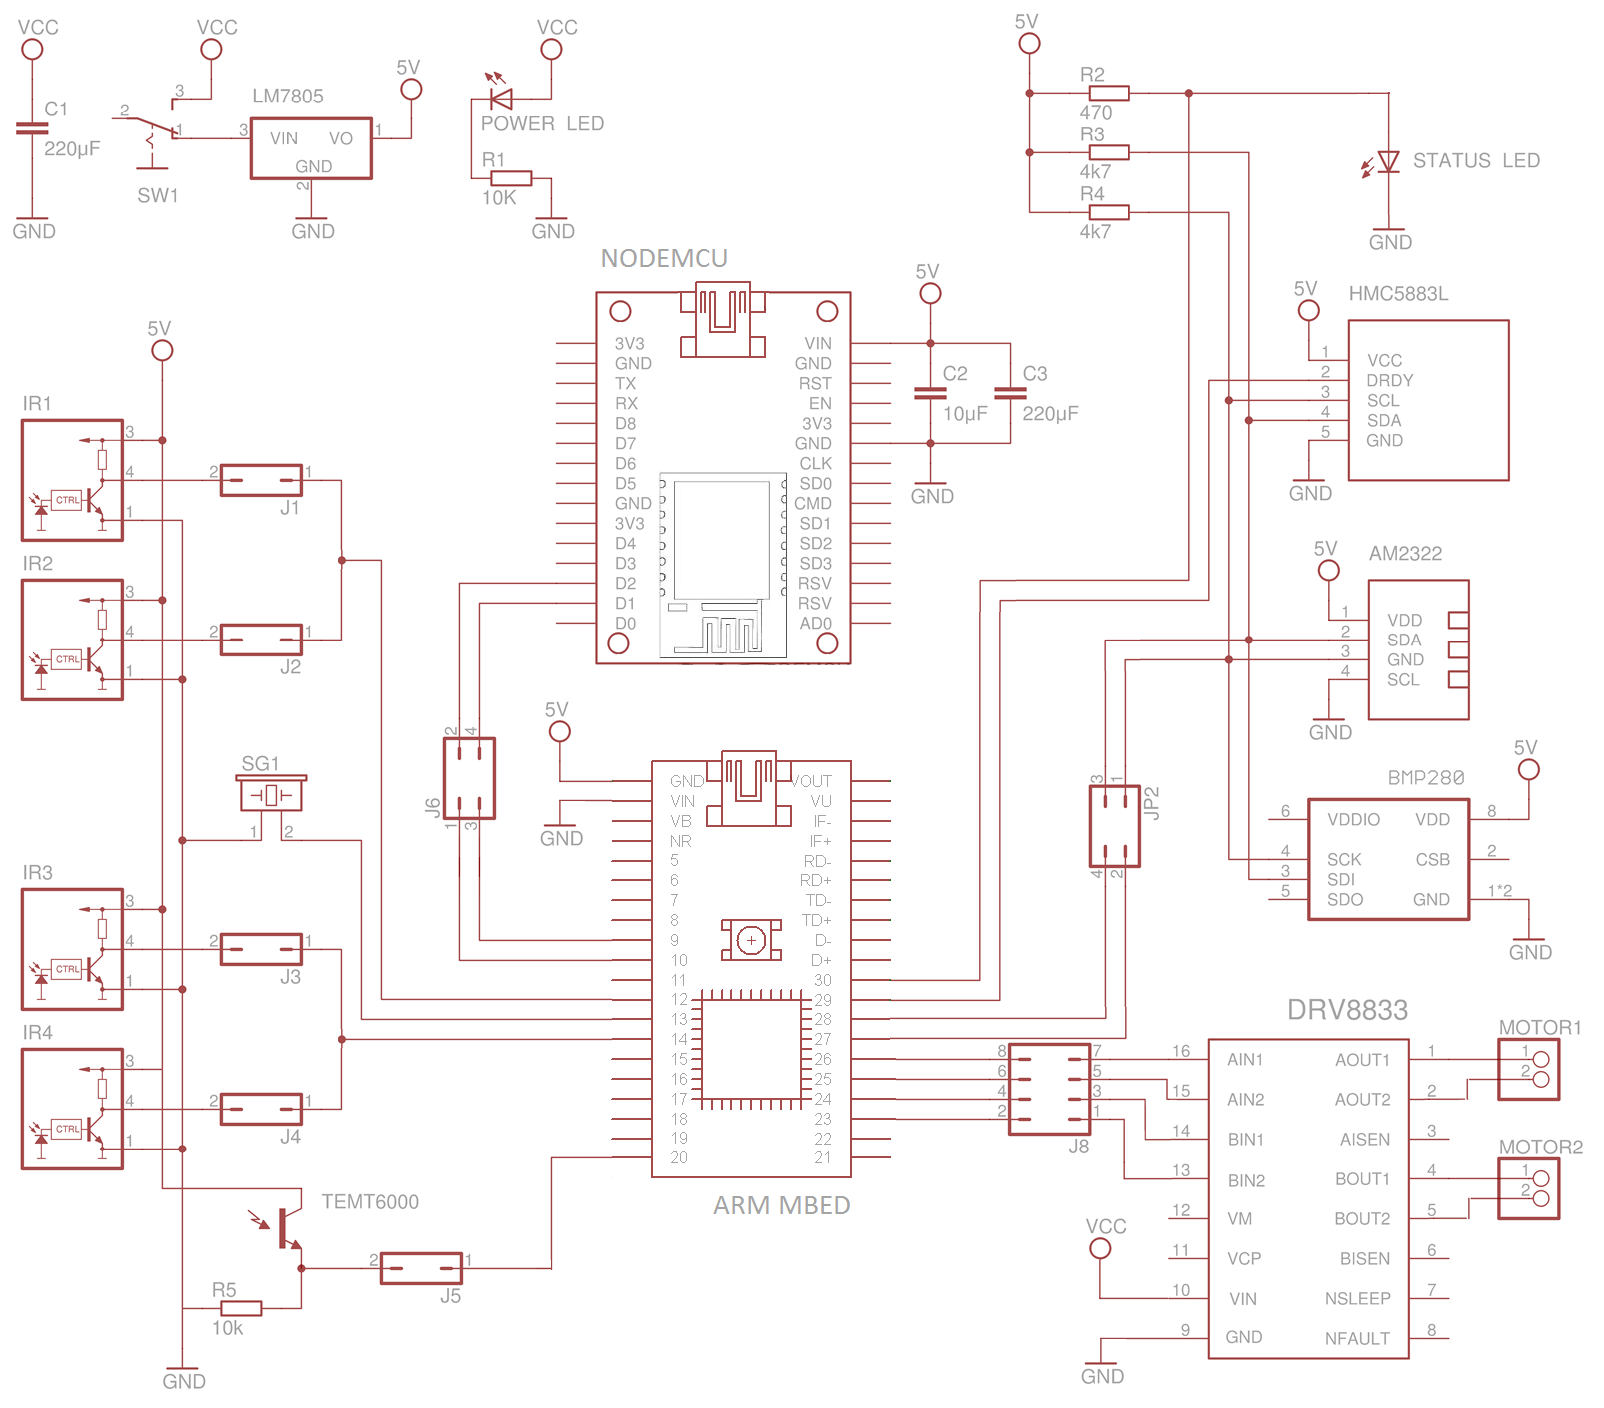
\includegraphics[width=\textwidth]{figuri/schema.png}
\end{appendices}

\end{document}